\documentclass[11pt,final,fleqn]{article}\usepackage[]{graphicx}\usepackage[]{color}
%% maxwidth is the original width if it is less than linewidth
%% otherwise use linewidth (to make sure the graphics do not exceed the margin)
\makeatletter
\def\maxwidth{ %
  \ifdim\Gin@nat@width>\linewidth
    \linewidth
  \else
    \Gin@nat@width
  \fi
}
\makeatother

\definecolor{fgcolor}{rgb}{0.345, 0.345, 0.345}
\newcommand{\hlnum}[1]{\textcolor[rgb]{0.686,0.059,0.569}{#1}}%
\newcommand{\hlstr}[1]{\textcolor[rgb]{0.192,0.494,0.8}{#1}}%
\newcommand{\hlcom}[1]{\textcolor[rgb]{0.678,0.584,0.686}{\textit{#1}}}%
\newcommand{\hlopt}[1]{\textcolor[rgb]{0,0,0}{#1}}%
\newcommand{\hlstd}[1]{\textcolor[rgb]{0.345,0.345,0.345}{#1}}%
\newcommand{\hlkwa}[1]{\textcolor[rgb]{0.161,0.373,0.58}{\textbf{#1}}}%
\newcommand{\hlkwb}[1]{\textcolor[rgb]{0.69,0.353,0.396}{#1}}%
\newcommand{\hlkwc}[1]{\textcolor[rgb]{0.333,0.667,0.333}{#1}}%
\newcommand{\hlkwd}[1]{\textcolor[rgb]{0.737,0.353,0.396}{\textbf{#1}}}%
\let\hlipl\hlkwb

\usepackage{framed}
\makeatletter
\newenvironment{kframe}{%
 \def\at@end@of@kframe{}%
 \ifinner\ifhmode%
  \def\at@end@of@kframe{\end{minipage}}%
  \begin{minipage}{\columnwidth}%
 \fi\fi%
 \def\FrameCommand##1{\hskip\@totalleftmargin \hskip-\fboxsep
 \colorbox{shadecolor}{##1}\hskip-\fboxsep
     % There is no \\@totalrightmargin, so:
     \hskip-\linewidth \hskip-\@totalleftmargin \hskip\columnwidth}%
 \MakeFramed {\advance\hsize-\width
   \@totalleftmargin\z@ \linewidth\hsize
   \@setminipage}}%
 {\par\unskip\endMakeFramed%
 \at@end@of@kframe}
\makeatother

\definecolor{shadecolor}{rgb}{.97, .97, .97}
\definecolor{messagecolor}{rgb}{0, 0, 0}
\definecolor{warningcolor}{rgb}{1, 0, 1}
\definecolor{errorcolor}{rgb}{1, 0, 0}
\newenvironment{knitrout}{}{} % an empty environment to be redefined in TeX

\usepackage{alltt}

% basic packages
\usepackage[T1]{fontenc}
\usepackage[margin=1in] { geometry }
\usepackage{amssymb,amsmath, bm}
\usepackage{verbatim}
\usepackage[latin1]{inputenc}
%\usepackage[OT1]{fontenc}
\usepackage{setspace}
\usepackage{natbib}
\usepackage{enumitem}
\usepackage[hyphens,spaces,obeyspaces]{url}
\usepackage[font={bf}]{caption}
%\usepackage{pgfplots}
%\usepackage[font={bf}]{caption}
\usepackage{setspace}
\usepackage{latexsym}
%\usepackage{euscript}
\usepackage{graphicx}
\usepackage{marvosym}
%\usepackage[varg]{txfonts}  Older version of ``g'' in math.
\usepackage{pdflscape}
\usepackage{algorithm}

% bibliography packages
\usepackage{natbib}
\bibpunct{(}{)}{;}{a}{}{,}
\bibliographystyle{apa}
\renewcommand{\bibname}{References}

% hyperref options
\usepackage{color}
\usepackage{hyperref}
\usepackage{xcolor}
\hypersetup{
    colorlinks,
    linkcolor={blue!50!black},
    citecolor={blue!50!black},
    urlcolor={blue!80!black}
}
\newcommand*{\Appendixautorefname}{Appendix}
\renewcommand*{\sectionautorefname}{Section}
\renewcommand*{\subsectionautorefname}{Section}
\renewcommand*{\subsubsectionautorefname}{Section}
\newcommand{\subfigureautorefname}{\figureautorefname}
\newcommand{\aref}[1]{\hyperref[#1]{Appendix~\ref{#1}}}
\newcommand{\algorithmautorefname}{Algorithm}

% packages for tables
\usepackage{longtable}
\usepackage{booktabs, threeparttable}
\usepackage{threeparttablex}
\usepackage{tabularx}
% dcolumn package
\usepackage{dcolumn}
\newcolumntype{.}{D{.}{.}{-1}}
\newcolumntype{d}[1]{D{.}{.}{#1}}
\captionsetup{belowskip=10pt,aboveskip=-5pt}
\usepackage{multirow}
% rotating package
\usepackage[figuresright]{rotating}
\usepackage{pdflscape}
\usepackage{subcaption}
\usepackage{caption} 
\captionsetup[table]{skip=5pt}

% packages for figures
\usepackage{grffile}
\usepackage{afterpage}
\usepackage{float}
\usepackage[section]{placeins}
\usepackage[export]{adjustbox}

% theorem package
\usepackage{theorem}
\theoremstyle{plain}
\theoremheaderfont{\scshape}
\newtheorem{theorem}{Theorem}
\newtheorem{assumption}{Assumption}
\newtheorem{lemma}{Lemma}
\newtheorem{proposition}{Proposition}
\newtheorem{remark}{Remark}
\newcommand{\qed}{\hfill \ensuremath{\Box}}
\newcommand\indep{\protect\mathpalette{\protect\independenT}{\perp}}
\DeclareMathOperator{\sgn}{sgn}
\DeclareMathOperator{\tr}{tr}
\DeclareMathOperator{\argmin}{arg\min}
\DeclareMathOperator{\argmax}{arg\max}
\def\independenT#1#2{\mathrel{\rlap{$#1#2$}\mkern2mu{#1#2}}}
\providecommand{\norm}[1]{\lVert#1\rVert}
\renewcommand\r{\right}
\renewcommand\l{\left}
\newcommand\E{\mathbb{E}}
\newcommand\dist{\buildrel\rm d\over\sim}
\newcommand\iid{\stackrel{\rm i.i.d.}{\sim}}
\newcommand\ind{\stackrel{\rm indep.}{\sim}}
\newcommand\cov{{\rm Cov}}
\newcommand\var{{\rm Var}}
\newcommand\SD{{\rm SD}}
\newcommand\bone{\mathbf{1}}
\newcommand\bzero{\mathbf{0}}

% file paths and definitions
\makeatletter
\newcommand*\ExpandableInput[1]{\@@input#1 }
\makeatother

% spacing 
\usepackage[compact]{titlesec}
\setlength{\parindent}{0pt}
\setlength{\parskip}{6pt plus 2pt minus 1pt}

% appendix settings
\usepackage[toc,page,header]{appendix}
\renewcommand{\appendixpagename}{\centering Appendices}
\usepackage{chngcntr}
\usepackage{etoolbox}
\usepackage{lipsum}

% new commands
\newcommand\CPP{{C\texttt{++}}}
\newcommand\R{{\textsf{R}}}


% title
\title{A Description of the IVI-RA Model}
\author{Devin Incerti\footnote{Innovation and Value Initiative} \and Jeroen P. Jansen\footnote{Innovation and Value Initiative}}
\date{\today}
\IfFileExists{upquote.sty}{\usepackage{upquote}}{}
\begin{document}
\maketitle

\begingroup
 \hypersetup{linkcolor=black} \tableofcontents
 \listoffigures
 \listoftables
\endgroup



\section{Overview}\label{overview}

This document describes version 0.1 of IVI's rheumatoid arthritis (RA) cost-effectiveness model. The IVI-RA model is an individual patient simulation (IPS) that simulates patients one at a time. The model reflects a range of perspectives (e.g., health care sector, societal) and structural assumptions. All told, there are 280 different model structures, which allows analysts to account for structural uncertainty. Parameter uncertainty is quantified with probabilistic sensitivity analysis (PSA).

The model is available as an \href{https://cran.r-project.org/}{\R{}} package with documentation available \href{https://innovationvalueinitiative.github.io/IVI-RA/index.html}{online}. The source code can be viewed or downloaded at our \href{https://github.com/InnovationValueInitiative/IVI-RA}{GitHub repository}. The IPS was primarily written in \CPP{} so that PSA and analyses of structural uncertainty can be run in a reasonable amount of time. The model can either be run using \R{} (see \href{https://innovationvalueinitiative.github.io/IVI-RA/index.html}{documentation}) or \href{http://www.shinyapps.io/}{online} with our user-friendly R Shiny web application. 

This document is structured as follows. We begin by discussing treatment strategies that can be modeled in \autoref{sec:treatments}. \autoref{sec:model-structures} outlines the competing model structures. \autoref{sec:data-parameters} describes the statistical techniques used to estimate the model parameters and the data sources used. \autoref{sec:populations} examines the data needed to define a population and run an analysis. Finally, \autoref{sec:sim-uncertainty} describes the simulation techniques used to implement the RA family of models and quantify uncertainty.

\section{Treatment strategies}\label{sec:treatments}
The primary purpose of the model is to evaluate the cost-effectiveness of treatments for RA. Since patients typically use multiple treatments over a lifetime, the model is capable of simulating a treatment sequence of any arbitrary length. Treatments that can be included in a sequence include conventional disease-modifying anti-rheumatic drugs (cDMARDs) such as methotrexate as well as the following biologic DMARDS (bDMARDs):

\begin{itemize}
\item \textbf{Tumor necrosis factor (TNF) inhibitors}: etanercept, adalimumab, certolizumab, golimumab
\item \textbf{non-TNF inhibitors}: abatecept, tocilizumab, rituximab
\item \textbf{Janus kinase/signal transducers and activators of transcription (JAK/STAT) inhibitors}: tofacitinib
\end{itemize}

At the end of a sequence, patient switch to non-biologic therapy (NBT), which encompasses a range of therapies that do not affect the rate of disease progression and are not associated with adverse events. 

\section{Competing model structures}\label{sec:model-structures}
The IVI-RA model is a discrete-time IPS with 6 month cycles that can be run using a number of different model structures. Like most RA cost-effectiveness models, the model measures changes in disease severity using the Health Assessment Questionnaire (HAQ) Disability Index score \citep{tosh2011sheffield, carlson2015economic, stephens2015modelling, stevenson2016adalimumab, icer2017tim, stevenson2017cost}. In particular, at the start of the simulation, each patient is assigned a baseline HAQ score. Subsequently, the impact of the disease measured by the HAQ trajectory over time is modeled as a function of a sequence of treatments (\autoref{fig:haq-structure}). In the absence of treatment, HAQ deteriorates at a certain rate as depicted by the dashed line in the figure. Treatment is separated into two distinct phases: an initial phase of up to 6 months, consistent with data reported from randomized controlled trials (RCTs), and a maintenance phase thereafter until discontinuation. 

\begin{figure}
\centering
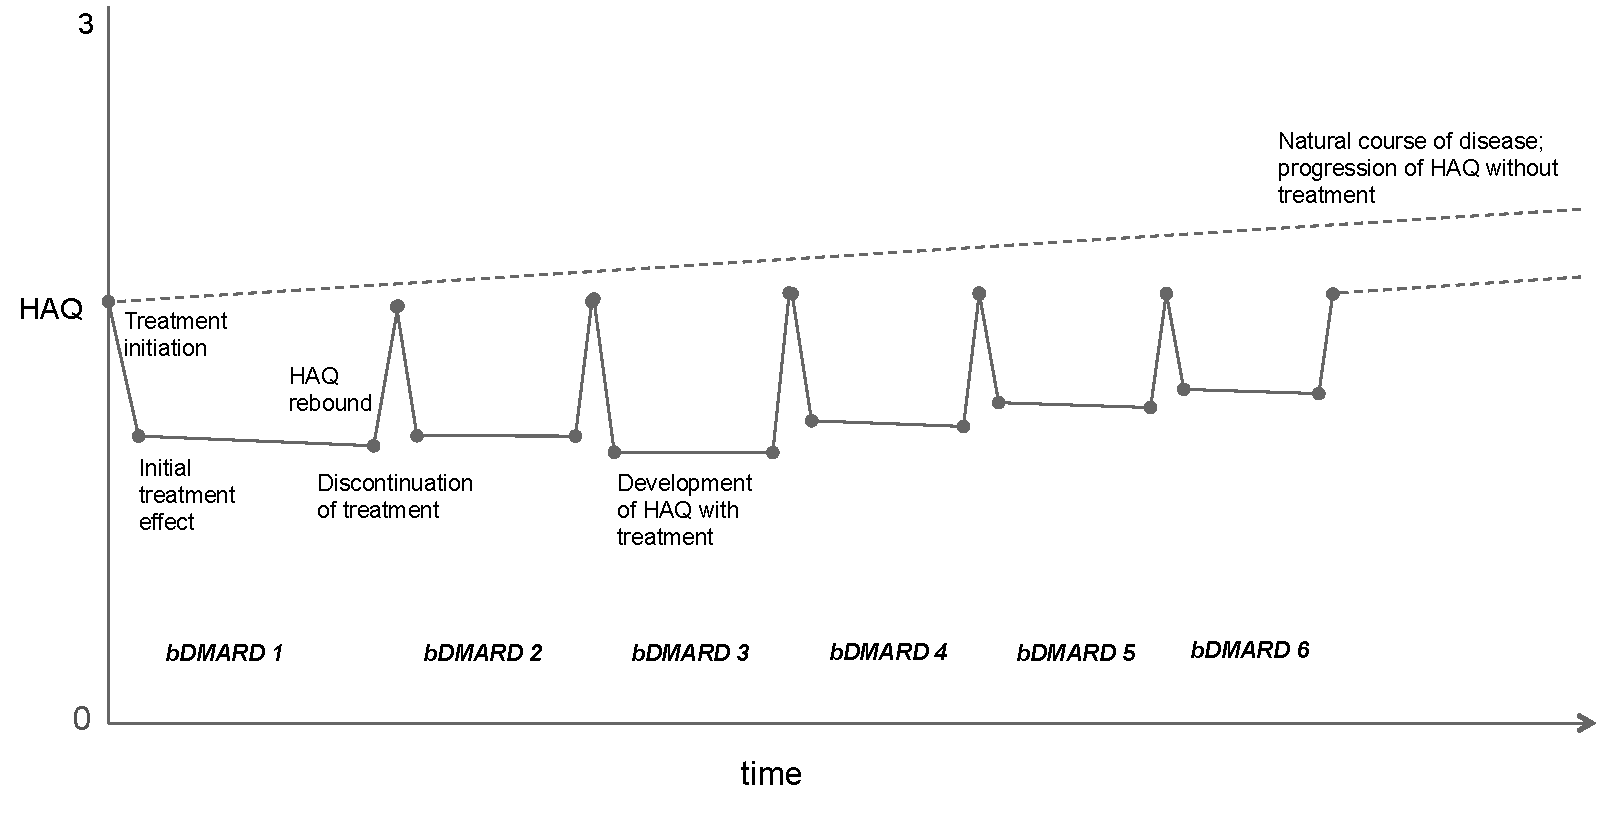
\includegraphics[max size={\textwidth}{\textheight}]{figs/haq-structure.pdf}
\caption{Model structure regarding development of HAQ with sequential
biologic treatment}\label{fig:haq-structure}
\end{figure}

During the initial treatment phase HAQ is modeled as a change from baseline. Three possible model structures labeled \textbf{H1-H3} are possible. In \textbf{H1}, treatment influences HAQ through its effect on the American College of Rheumatology (ACR) response criteria, which is similar to the structure used in other US based cost-effectiveness models \citep[e.g.][]{carlson2015economic, icer2017tim}. ACR response is measured using four mutually exclusive categories: no response (defined as less than 20\% improvement), ACR 20-50\% improvement, ACR 50-70\% improvement, and ACR 70\% improvement or greater. The rationale for using ACR response rather than HAQ directly is that the evidence base relating treatment to ACR response is larger than the evidence based relating treatment to HAQ. \textbf{H2} follows the National Institute for Health and Care Excellence (NICE) cost-effectiveness model \citep{stevenson2016adalimumab, stevenson2017cost} and models the effect of treatment on HAQ indirectly through its effect on ACR response and, in turn, the three categories of the European League Against Rheumatism (EULAR) response (no response, moderate response, or good response). Finally, since modeling the effect of treatment on HAQ through intermediary variables may mediate treatment response, in \textbf{H3}, treatment impacts HAQ directly. The three scenarios are summarized below: 

\begin{itemize}
\item \textbf{H1}: Treatment $\rightarrow$ ACR $\rightarrow$ HAQ
\item \textbf{H2}: Treatment $\rightarrow$ ACR $\rightarrow$ EULAR $\rightarrow$ HAQ
\item \textbf{H3}: Treatment $\rightarrow$ HAQ
\end{itemize}

The probability of switching treatment during the initial treatment phase is modeled using 6 possible structures labeled \textbf{S1-S5}. \textbf{S1} follows a common approach where ACR non-responders discontinue treatment \citep[e.g.][]{carlson2015economic, icer2017tim}. One drawback of this approach is that it is not consistent with current treat-to-target guidelines in the United States \citep{singh20162015}. \textbf{S2} and \textbf{S3} consequently model treatment switching as a function of disease activity (remission, low, moderate, high) \citep{anderson2012rheumatoid}. ACR response predicts the change in disease activity from baseline which, along with baseline disease activity, predicts absolute disease activity. The probability of switching treatment is increasing in the severity of disease (i.e., the probability is lowest in remission and greatest with high disease activity). In \textbf{S2} disease activity is measured using the Disease Activity Score with 28-joint counts (DAS28) \citep{prevoo1995modified} and in \textbf{S3} disease activity is measured using the Simplified Disease Activity Index (SDAI) \citep{smolen2003simplified, aletaha2005simplified}. We considered the Clinical Disease Activity Index (CDAI) as well, but do not have data linking ACR response to CDAI.

\textbf{S4} is similar to \textbf{S2} and \textbf{S3}, but models the effect of treatment on changes in DAS28 directly, rather than indirectly through ACR response. We also aimed to model the direct effect of treatment on SDAI and CDAI, but sufficient clinical trial data is not available. Finally, since in the UK, the EULAR response is recommended by the British Society for Rheumatology and the British Health Professionals in Rheumatology \citep{deighton2010bsr}, \textbf{S5} is based on EULAR response. In particular, following the NICE model, we assume that EULAR non-responders discontinue treatment while moderate and good responders continue treatment \citep{stevenson2016adalimumab}. The reasoning is that rules stipulated by NICE require a DAS28 improvement of more than 1.2 to continue treatment which is associated with moderate or good EULAR response. All 5 treatment switching scenarios are summarized below: 

\begin{itemize}
\item \textbf{S1:} Treatment $\rightarrow$ ACR $\rightarrow$ Switch
\item \textbf{S2:} Treatment $\rightarrow$ ACR $\rightarrow$ $\Delta$DAS28 $\rightarrow$ DAS28 $\rightarrow$ Switch 
\item \textbf{S3:} Treatment $\rightarrow$ ACR $\rightarrow$ $\Delta$SDAI $\rightarrow$ SDAI $\rightarrow$ Switch 
\item \textbf{S4:} Treatment $\rightarrow$ $\Delta$DAS28 $\rightarrow$ DAS28 $\rightarrow$ Switch 
\item \textbf{S5:} Treatment $\rightarrow$ ACR $\rightarrow$ EULAR $\rightarrow$ Switch
\end{itemize}

Not all model structures \textbf{S1-S5} can be used with each of \textbf{H1-H3}. If \textbf{H1} is used, then \textbf{S1-S4} are available, but \textbf{S5} is not because EULAR response is not simulated. In \textbf{H2}, \textbf{S1-S5} are all available while in \textbf{H3} only \textbf{S4} can be used since neither ACR or EULAR response are simulated. The 10 possible model structures and the number of each structure are outlined in \autoref{tbl:initial-model-structure}.  

\begin{table}[!ht] 
\begin{center}
\begin{threeparttable}
\caption{Model structures for initial treatment phase} \label{tbl:initial-model-structure}
\begin{tabularx}{\textwidth}{@{\extracolsep{\fill}}lccccc}
\hline
\multicolumn{1}{l}{} & \multicolumn{1}{c}{S1} & \multicolumn{1}{c}{S2} & \multicolumn{1}{c}{S3} & \multicolumn{1}{c}{S4} & \multicolumn{1}{c}{S5}  \\
\hline
H1 & 1 & 2 & 3 & 4 & - \\
H2 & 5 & 6 & 7 & 8 & 9 \\
H3 & - & - & - & 10 & - \\
\hline
\end{tabularx}
\scriptsize
Notes: Rows denote the model structure used to relate treatment to HAQ and columns denote the model structure used to predict treatment switching. Each number denotes a unique model structure (i.e. 1 corresponds to H1 and S1 and 8 corresponds to H2 and S4) and the "-" denotes a model structure combination that is not possible. There are 10 possible model structures for the initial treatment phase. 
\end{threeparttable}
\end{center}
\end{table}


In the maintenance phase, two model structures can be used to simulate the long-term progression of HAQ. First, as is common in cost-effectiveness analyses of therapies for RA, HAQ is assumed to progress at a constant linear rate over time \citep[see][]{tosh2011sheffield, wailoo2008biologic}. However, since emerging evidence suggests that the rate of HAQ progression is non-linear \citep{gibson2016haq}, our second scenario simulates HAQ progression using a non-linear mixture model \citep{norton2014health} with 4 distinct HAQ trajectories and a rate of HAQ progression that decreases over time within each trajectory. Upon discontinuation of treatment, the HAQ score rebounds by a proportion of the improvement experienced at the end of the initial 6-month period with that treatment.

The duration of the maintenance phase (i.e., time to discontinuation of maintenance treatment) is simulated using parametric time-to-event distributions. When structure \textbf{S5} is used, the time-to-event distributions are stratified by EULAR response category. Patients with good response at the end of the initial treatment phase stay on treatment longer, on average, than patients with a moderate response. In contrast, when \textbf{S1} is used, time to treatment discontinuation is simulated using a single time-to-event curve because we have been unable to obtain curves stratified by ACR response categories. Likewise, when \textbf{S2-S4} we use a single time-to-event curve because we have not obtained curves stratified by disease activity level. In each case, time to discontinuation can be simulated using one of seven possible distributions (exponential, Weibull, Gompertz, normal, gamma, log-logistic, generalized gamma).

In line with \citet{stevenson2016adalimumab} the adverse events included in the model are limited to serious infections; we assume that only serious infections have a significant cost impact and increased risk over background rates to be meaningful to include \citep{ramiro2017safety}. While on a treatment, a patient experiences a serious infection if the individual's sampled time to the adverse event is shorter than the sampled time to treatment discontinuat on.

Baseline HAQ scores (and changes in HAQ scores from baseline) are used to determine mortality relative to age/sex specific rates for the US general population (assumed to have a HAQ score of 0). Treatment therefore has an indirect effect on mortality through its effect on HAQ. 

Individual HAQ scores at a particular point in time were also used to simulate EQ-5D utility scores (0-1 range), which, in turn, were used to simulate quality-adjusted life-years (QALYs). However, since a number of different methods have been used to convert HAQ into utility, our model contains two different possible mapping algorithms. Our preferred algorithm is the \citet{alava2013relationship} mixture model, which uses a much larger sample size than other statistical models and has been shown to have better predictive accuracy. Other algorithms are typically estimated using clinical trial data \citep[e.g.][]{carlson2015economic, stephens2015modelling} and consequently have limited generalizability. The second utility algorithm available within our model is based on a linear regression analyis of real-world data by \citet{wailoo2006modeling} that has been used in a few previous cost-effectiveness analyses \citep[e.g.][]{wailoo2008biologic, icer2017tim}. 

Annnual hospitalization days and productivity losses are simulated as a function of HAQ. Health sector costs considered in the models are related to drug acquisition and administration, adverse events, general management of RA, and hospitalization. Non-health sector costs considered are limited to work related productivity loss.

Patient preferences for treatment attributes have a direct effect on long-term treatment duration and utility. Patients with treatments that more closely match their preferences have longer treatment duration and higher utility. Treatment attributes that are incorporated into the models include route of administration and frequency of administration.

The flow diagram in \autoref{fig:flow-diagram} describes the flow of a single patient through the simulation. Each patient begins the simulation by initiating treatment and ends the simulation with death. The rectangles in the figure represent ``processes'' determining the effect of treatment on disease progression and the diamonds represent ``decisions'' that determine whether a patient will switch to a new treatment.

\begin{figure}
\centering
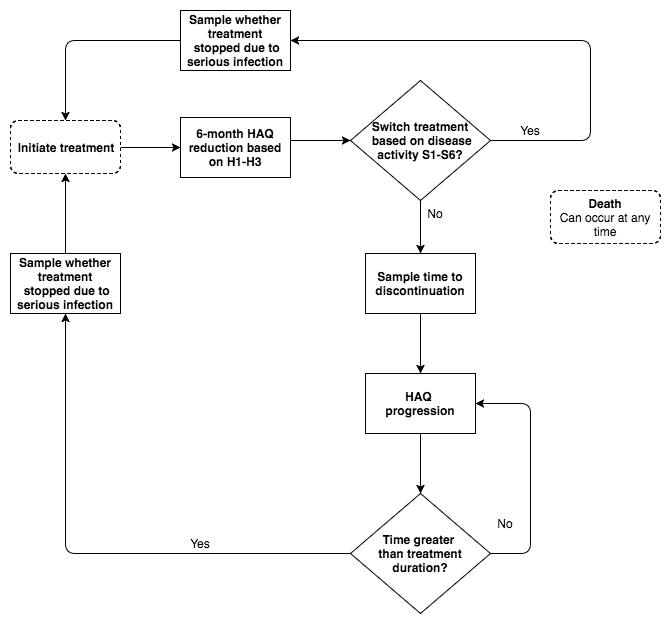
\includegraphics[max size={\textwidth}{\textheight}]{figs/flow-diagram.png}
\caption{Flow diagram of the simulation for a single
patient}\label{fig:flow-diagram}
\end{figure}

The influence diagram in \autoref{fig:influence-diagram} summarizes the assumed structural relationships among different variables in the model. Each arrow represents the direct effect of one parameter on another. Dashed lines represent relationships that depend on the structural assumptions used. \autoref{subfig:treatment-effects} focuses on the effect of treatment on disease progression and adverse events while \autoref{subfig:model-outcomes} looks at the variables influencing the primary health and cost outcomes. 

Model outcomes depend on patient characteristics, which have a direct effect on HAQ progression, mortality, and utility. The primary health outcome is the quality-adjusted life-year (QALY) which depends on mortality and utility. Total costs consist of health care sector costs and productivity losses. The components of health sector costs include drug acquisition and administration costs, general management and monitoring costs, adverse event costs, and hospitalization costs  Analyses from a societal perspective would include productivity losses while analyses from a health care sector perspective would not. The value of treatment is estimated using the net-monetary benefit (NMB), which is calculated by multiplying QALYs by a willingness to pay threshold and subtracting costs ($NMB = QALYS \cdot WTP - Costs$). 

\begin{figure}
\centering
\begin{subfigure}{\textwidth}
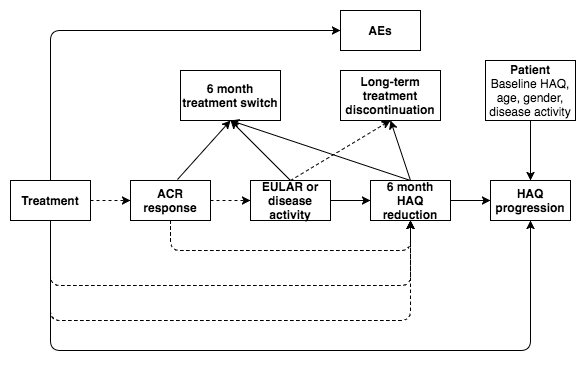
\includegraphics[width=\textwidth]{figs/influence-diagram-a.png}
\caption{Treatment effects} \label{subfig:treatment-effects}
\end{subfigure}
\begin{subfigure}{\textwidth}
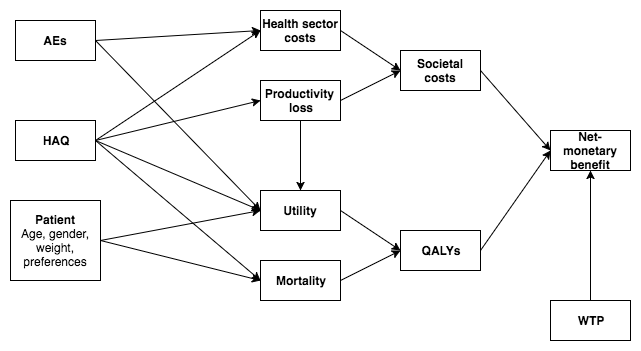
\includegraphics[width=\textwidth]{figs/influence-diagram-b.png}
\caption{Model outcomes} \label{subfig:model-outcomes}
\end{subfigure}
\caption{Influence diagram outlining structural relationships}\label{fig:influence-diagram}
\begin{minipage}{\linewidth}
\footnotesize
Notes: ACR: American College of Rheumatology; EULAR: European League Against Rheumatism; HAQ: Health Assessment Questionnaire; QALY: AEs: adverse events; QALYs: quality-adjusted life-years; WTP: willingness to pay. Disease activity refers to the Disease Activity Score with 28-joint counts (DAS28) or the Simplified Disease Activity Index (SDAI).
\end{minipage}
\end{figure}

\autoref{tbl:competing-structures} summarizes the competing model structures, which are conditional on the perspective of the decision maker. In total, there are 10 x 2 x 7 x 2 = 280 possible model structures.

\renewcommand{\arraystretch}{1.5}

\begin{table}[!ht]
\begin{center}
\begin{threeparttable}
\caption{Competing model structures} \label{tbl:competing-structures}
\begin{tabular}{p{0.80\linewidth}p{0.20\linewidth}}
\hline
\multicolumn{1}{c}{Component of model structure} & \multicolumn{1}{c}{Possible combinations} \\
\hline
Initial effect of treatment on HAQ (\textbf{H1-H3}) and switching (\textbf{S1-S6}) & 10  \\
HAQ progression linear or non-linear & 2 \\
Probability distribution for treatment duration & 7 \\
Utility algorithm & 2 \\
\hline
\end{tabular}
\end{threeparttable}
\end{center}
\end{table}\renewcommand{\arraystretch}{1}

\section{Populations}\label{sec:populations}

\section{Source data and parameter estimation}\label{sec:data-parameters}
\subsection{Change in HAQ during initial treatment phase}\label{initial-change-haq}
\subsubsection{H1: Treatment $\rightarrow$ ACR $\rightarrow$ HAQ}



\begin{table}[!ht]
\begin{center}
\begin{threeparttable}
\caption{Relationship between ACR response and change in HAQ at 6 months} \label{tbl:acr2haq}
\begin{tabularx}{\textwidth}{@{\extracolsep{\fill}}lcc}
\hline
\multicolumn{1}{l}{} & \multicolumn{2}{c}{HAQ change} \\
\cmidrule{2-3} 
\multicolumn{1}{c}{ACR response} & \multicolumn{1}{c}{Mean} & \multicolumn{1}{c}{Standard error} \\
\hline
\ExpandableInput{tables/acr2haq.txt}
\hline
\end{tabularx}
\scriptsize
Source: \citet{carlson2015economic}
\end{threeparttable}
\end{center}
\end{table}

\subsubsection{H2: Treatment $\rightarrow$ ACR $\rightarrow$ EULAR $\rightarrow$ HAQ}

Treatment effects for bDMARD \emph{naive} patients at 6 months are estimated using a Bayesian network meta-analysis (NMA) of published
randomized controlled trials (RCTs) (see \autoref{sec:tech-nma-initial}). Two primary endpoints were considered: ACR 20/50/70 response and HAQ.
. In one version of the model structure, EULAR response categories are used to determine treatment continuation and duration. ACR responses from the NMA were translated into EULAR response probabilities based on evidence of their relationship reported in \citet{stevenson2016adalimumab} and obtained from the US Veterans Affairs Rheumatoid Arthritis (VARA) registry (\autoref{tbl:acr2eular}).



\begin{table}[!ht]
\begin{center}
\begin{threeparttable}
\caption{Relationship between ACR response and EULAR response} \label{tbl:acr2eular}
\begin{tabularx}{\textwidth}{@{\extracolsep{\fill}}lcccc}
\hline
\multicolumn{1}{l}{} & \multicolumn{3}{c}{EULAR response} \\
\cmidrule{2-4} 
\multicolumn{1}{c}{ACR response} & \multicolumn{1}{c}{None} & \multicolumn{1}{c}{Moderate} & \multicolumn{1}{c}{Good} \\
\hline
\ExpandableInput{tables/acr2eular.txt}
\hline
\end{tabularx}
\scriptsize
Notes: The VARA registry is a multicentre, US database of veterans age 19 and older. Each cell represents the number of patients in the 
database in a given category. 
\end{threeparttable}
\end{center}
\end{table}



The model structure allows treatment to impact HAQ either directly or indirectly through its effect on ACR response. In the indirect case, ACR response first affects EULAR response or SDAI using the evidence reported in \autoref{tbl:acr2eular}, which, in turn, affects HAQ. The relationship between EULAR response and HAQ is based on analyses conducted by \citet{stevenson2016adalimumab} using the BSRBR database. Their analysis is based on predictions from a mixture model with covariates set to sample means. Moderate and good EULAR response are associated with -0.317 (SE = 0.048) and -0.672 (SE = 0.112) changes in HAQ scores respectively. The impact of treatment on ACR response, EULAR response, and HAQ (given their ACR and EULAR responses) is shown in \autoref{tbl:initial-haq}.



\begin{landscape}
\begin{table}[!ht]
\begin{center}
\begin{threeparttable}
\caption{Response at 6 months for 1st line treatment} \label{tbl:initial-haq}
\scriptsize
\begin{tabular}{lrrrrrrrr}
\hline
\multicolumn{1}{c}{} & \multicolumn{4}{c}{ACR response} & \multicolumn{3}{c}{EULAR response} & \multicolumn{1}{c}{\multirow{2}{*}{Mean HAQ}}\\
\cmidrule(lr){2-5} \cmidrule(lr){6-8}
\multicolumn{1}{l}{Treatment} & \multicolumn{1}{c}{$<$20} & \multicolumn{1}{c}{20-50} & \multicolumn{1}{c}{50-70}  & \multicolumn{1}{c}{70+}   & \multicolumn{1}{c}{None} & \multicolumn{1}{c}{Moderate}  & \multicolumn{1}{c}{Good}  & \multicolumn{1}{c}{decrease}\\
\hline
\ExpandableInput{tables/initital_response.txt}
\hline
\end{tabular}
\tiny
Notes: 95\% credible intervals are in parentheses. Estimates are based on 6-month simulations of 1,000 patients and 1,000 parameters sets for each therapy. cDMARDs = conventional disease-modifying antirheumatic drugs; MTX = methotrexate; ABT IV = abatacept intravenous; ADA = adalimumab; ETN = etanercept; GOL = golimumab; IFX = infliximab; TCZ = tocilizumab; CZP = certolizumab pegol; ABT SC = abatacept subcutaneous; RTX = rituximab; TOF = tofacitinib. ACR = American College of Rheumatology; EULAR = European League Against Rheumatism; HAQ = Health Assessment Questionnaire. 
\end{threeparttable}
\end{center}
\end{table}
\end{landscape}

\subsubsection{H3: Treatment $\rightarrow$ HAQ}

\subsection{Switching during the initial treatment phase}

\subsection{HAQ progression in the absence of bDMARD
treatment}\label{haq-progression-in-the-absence-of-bdmard-treatment}

The natural course of HAQ progression in the absence of bDMARDs develops over time according to an estimated natural course for patients remaining on cDMARDs or following discontinuation of the last bDMARD of the sequence. The natural course of HAQ can either be assumed to change at a constant linear rate or be modeled using a non-linear mixture model. 

\subsubsection{Constant linear rate of progression} \label{sec:haq-linear-rate}
The rate of progression in the linear case is based on the observational study by \citet{wolfe2010loss}. They assessed the development of HAQ over time at six month intervals for up to 11 years among 3,829 RA patients who switched from non-biologic treatment to biologic treatment and participated in the National Data Bank for Rheumatic Diseases (NDB) longitudinal study of RA outcomes. The annual HAQ progression rate prior to biologic therapy was 0.031 (95\% confidence interval (95\%CI): 0.026 to 0.036) and is assumed to reflect the course of progression of HAQ in the absence of bDMARD.

Based on the same data, \citet{michaud2011treatment} reported overall and age-specific specific HAQ progression rates. The differences between the overall and age specific rates are as follows: \textless{}40: -0.020 (95\%CI: -0.0223 to -0.0177); 40-64: -0.008 (95\%CI: -0.0101 to -0.0059); \(\geq\) 65 0.017 (95\%CI: 0.0136 to 0.0204). These estimates are applied to the overall progression rate of 0.031 to obtain age specific HAQ progression rates.



\begin{table}[!ht]
\begin{center}
\begin{threeparttable}
\caption{Annual linear progression of HAQ in the absence of bDMARDs beyond 6 months} \label{tbl:haq-lprog}
\footnotesize
\begin{tabularx}{\textwidth}{@{\extracolsep{\fill}}lrrrl}
\hline
\multicolumn{2}{l}{} & \multicolumn{2}{c}{95\% CI} & \multicolumn{1}{l}{} \\
\cmidrule{3-4} 
\multicolumn{1}{l}{} & \multicolumn{1}{r}{Estimate} & \multicolumn{1}{r}{Lower} & \multicolumn{1}{r}{Upper} & \multicolumn{1}{l}{Reference} \\
\hline
Overall progression rate \\
\ExpandableInput{tables/haq-lprog-cdmards.txt}
Change in overall progression rate by age \\
\ExpandableInput{tables/haq-lprog-diff-byage.txt}
\hline
\end{tabularx}
\scriptsize
Notes: 95\% confidence intervals are calculated using a normal distribution. Confidence intervals for changes in HAQ progression rates by age assume no covariance between the overall progression rate and the age-specific rates reported by \citet{michaud2011treatment}.
\end{threeparttable}
\end{center}
\end{table}

\subsubsection{Non-linear mixture model} \label{sec:haq-mixture}

The rate of progression in the non-linear case is based on a mixture model approach that has increasingly been used to model HAQ progression over time \citep{stevenson2016adalimumab, norton2013trajectories, norton2014health}. These models suggest that different subgroups have distinct HAQ trajectories and that the rate of worsening of HAQ progression decreases over time. Parameter estimates are based on We use the statistical model estimated on the Early Rheumatoid Arthritis Cohort Study (ERAS) cohort, which has a high percentage of patients receiving methotrexate and a very small percentage receiving biologics. Following \citet{stevenson2016adalimumab}, explanatory variables in the statistical model that are not used in the IPS will be set to their mean values in the ERAS cohort. Uncertainty in the parameters of the mixture model are based on standard errors since \citet{norton2013trajectories} did not report the full covariance matrix needed to model the covariance between the parameters.

\subsection{HAQ trajectory with bDMARD maintenance treatment}
Based on the NDB longitudinal study, \citet{wolfe2010loss} estimated the overall annual HAQ progression rate among RA patients who had switched to biologic treatment at -0.001 (95CI: -0.004 to 0.002). In a separate analysis, also based on NDB data, \citet{michaud2011treatment} reported annual HAQ progression rates by treatment adjusted for baseline HAQ score, age, sex, education, smoking, BMI, comorbidity, and RA onset. The average HAQ rate among patients on a biologic was -0.001 as well, which instills confidence that the reported HAQ progression rates for different bDMARDs as reported by \citet{michaud2011treatment} can be directly compared with the overall annual HAQ progression rate of 0.031 reported by \citet{wolfe2010loss}. Accordingly, bDMARD specific HAQ progression rates by \citet{michaud2011treatment} are used in the model. For bDMARD treatments evaluated in the model for which no HAQ progression rate was reported by \citet{michaud2011treatment}, the overall biologic rate of -0.001 is used. 

\subsection{Duration of maintenance treatment}\label{duration-of-maintenance-treatment}
\subsubsection{Corrona Database}\label{sec:ttd-corrona}
\subsubsection{BSRBR Database}\label{sec:ttd-bsrbr}
Treatment duration as a function of EULAR response is estimated from survival curves based on analyses of the British Society for Rheumatology Biologics Registers (BSRBR) database \citep{stevenson2016adalimumab}. Seven parametric survival models (exponential, Weibull, Gompertz, gamma, log-logistic, lognormal, and generalized gamma) were estimated on individual patient data reconstructed from the BSRBR survival curves using the algorithm developed in \citet{guyot2012enhanced}. The Akaike Information Criteria (AIK) and Bayesian Information Criteria (BIC) of each model by EULAR response category (moderate, good) are shown in \autoref{tbl:ic-dur-eular}.



\begin{table}[!ht]
\begin{center}
\begin{threeparttable}
\caption{AIC and BIC for parametric models of treatment duration by EULAR response} \label{tbl:ic-dur-eular}
\begin{tabularx}{\textwidth}{@{\extracolsep{\fill}}lcccc}
\hline
\multicolumn{1}{l}{} & \multicolumn{2}{c}{Moderate EULAR response} & \multicolumn{2}{c}{Good EULAR response} \\
\cmidrule{2-3} \cmidrule{4-5}
\multicolumn{1}{l}{Distribution} & \multicolumn{1}{c}{AIC} & \multicolumn{1}{c}{BIC} & \multicolumn{1}{c}{AIC}  & \multicolumn{1}{c}{BIC}   \\
\hline
\ExpandableInput{tables/duration-bsrbr-ipdsurv-eular-ic.txt}
\hline
\end{tabularx}
\end{threeparttable}
\end{center}
\end{table}

One concern is that the BSRBR is representative of the UK but not the
US. As a result, we also estimate ``adjusted'' survival models that are
more representative of the US. The adjustment is made in six steps based
on an analysis of the Consortium of Rheumatology Researchers of North
America (Corrona) database.

\begin{enumerate}
\def\labelenumi{\arabic{enumi}.}
\item Calculate a hazard function based on a survival curve from an analysis
  of the Corrona database. In particular, reconstruct individual patient
  data from the survival curve \citet{guyot2012enhanced} and fit a
  spline-based survival model. Then use the spline-based model to
  estimate the hazard function $h(t)_{corrona}$.
\item Calculate a hazard function based on the BSRBR. To do so, first
  calculate hazard functions for both moderate and good EULAR responders
  using the same method described in step 1. Then calculate an overall
  hazard function with the proportion of moderate and good responders in
  the BSRBR analysis. Given that the number of moderate responders is
  \(5,492\) and the number of good responders is $2,417$ the overall
  hazard function is $h(t)_{bsrbr} = \frac{5,492}{7,909}h(t)_{bsrbr, moderate} + \frac{2,417}{7,909}h(t)_{bbsrbr, good}$.
\item At each point in time, calculate the ratio of the Corrona and BSRBR
  hazard functions: $HR(t) = h(t)_{corrona}/h(t)_{bbsrbr}$.
\item Apply the hazard ratio in step 3 to the BSRBR hazard functions for
  each EULAR response category. That is $h(t)_{bsrbr, moderate, adj} = h(t)_{bsrbr, moderate} \cdot HR(t)$ and $h(t)_{bsrbr, good, adj} = h(t)_{bsrbr, good} \cdot HR(t)$.
\item Generate survival curves using the hazard functions from step 4.
  Specifically, given a general hazard function $h(t)$, calculate the
  cumulative hazard functions, $H(t) = \int_{z = 0}^{t} h(z)dz$,
  convert this to a survival function using $S(t) = exp(-H(t))$, and
  reconstruct individual patient data using the survival curve.
\item Fit parametric survival models to the individual patient data
  generated in step 5.
\end{enumerate}

Both adjusted and unadjusted survival curves by EULAR response fit using
a generalized gamma distribution are shown in \autoref{fig:bsrbr-gg}. AIC
and BIC for the parametric models fit in step 6 do the adjusted
individual patient data are shwon in \autoref{tbl:ic-dur-adj-eular}.

\begin{figure}
\centering
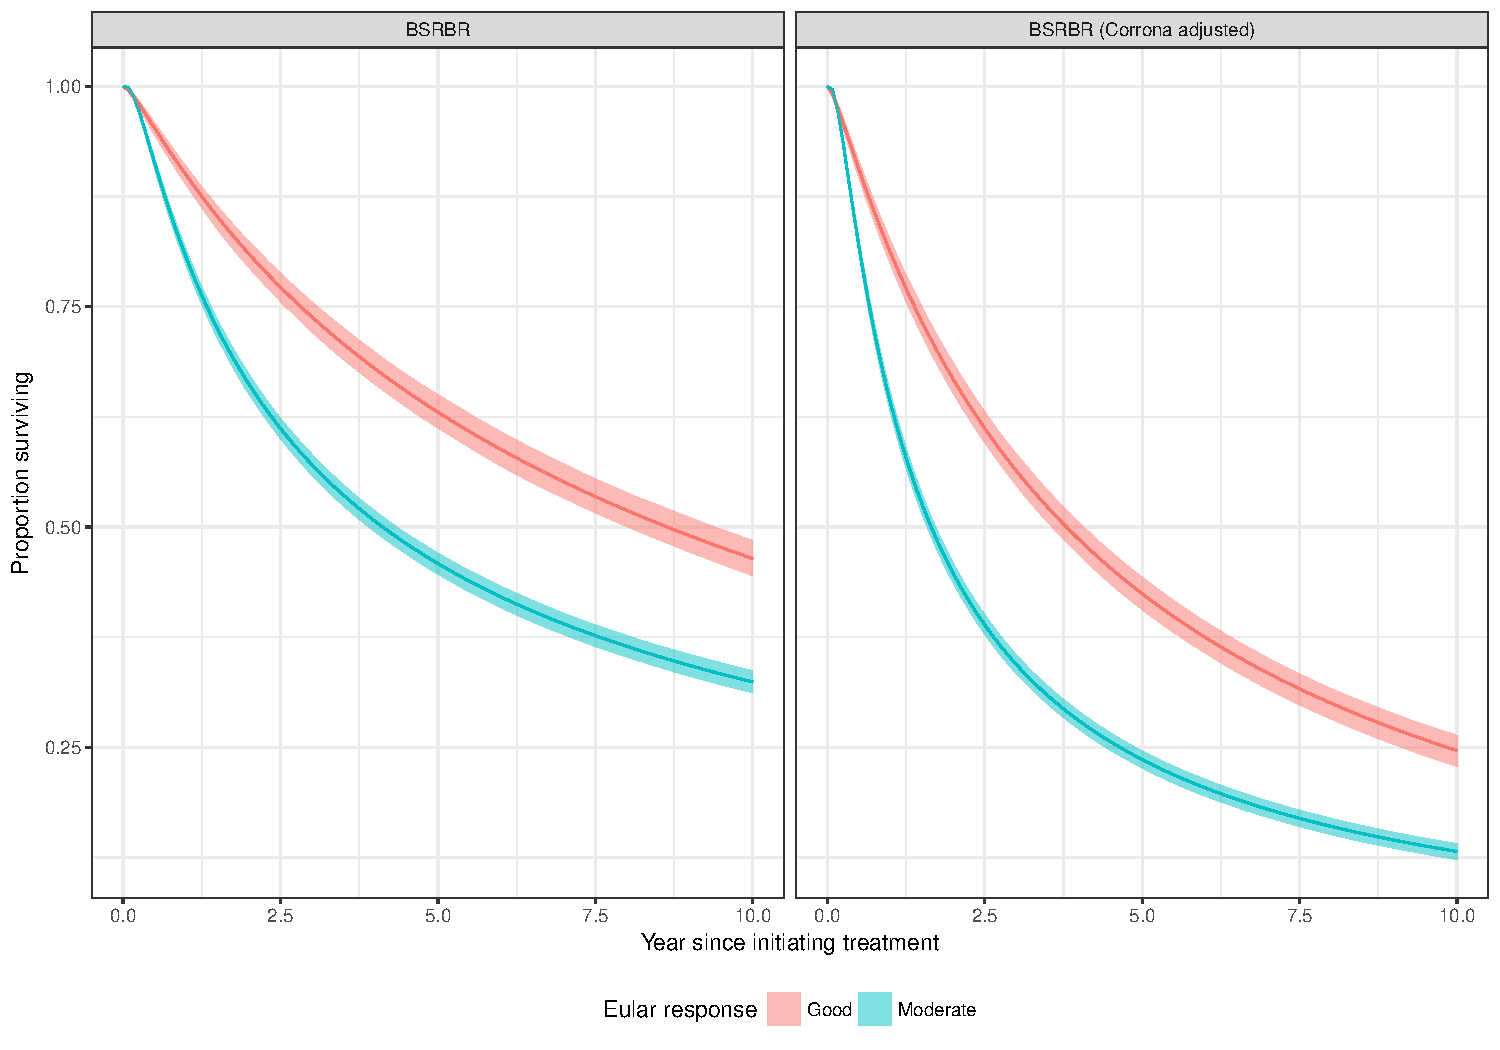
\includegraphics[max size={\textwidth}{\textheight}]{../../data-raw/figs/duration-bsrbr-ipdsurv-comp-gengamma-by-eular.pdf}
\caption{Generalized gamma survival curve of treatment duration using
reconstructed individual patient data based on analyses from Stevenson
et al. (2016) by EULAR response category}\label{fig:bsrbr-gg}
\end{figure}



\begin{table}[!ht]
\begin{center}
\begin{threeparttable}
\caption{AIC and BIC for Corrona adjusted parametric models of treatment duration by EULAR response} \label{tbl:ic-dur-adj-eular}
\begin{tabularx}{\textwidth}{@{\extracolsep{\fill}}lcccc}
\hline
\multicolumn{1}{l}{} & \multicolumn{2}{c}{Moderate EULAR response} & \multicolumn{2}{c}{Good EULAR response} \\
\cmidrule{2-3} \cmidrule{4-5}
\multicolumn{1}{l}{Distribution} & \multicolumn{1}{c}{AIC} & \multicolumn{1}{c}{BIC} & \multicolumn{1}{c}{AIC}  & \multicolumn{1}{c}{BIC}   \\
\hline
\ExpandableInput{tables/duration-bsrbr-ipdsurv-eular-adjusted-ic.txt}
\hline
\end{tabularx}
\end{threeparttable}
\end{center}
\end{table}

\subsection{Rebound post treatment}
Since no data exists on the size of the HAQ rebound post treatment, we vary its size as a proportion of the initial 6-month HAQ decline. 1 is used as an upper bound, which implies that the HAQ rebound is equal to the improvement experienced at the end of the initial 6-month period with that treatment. 0.5 is used as a lower bound based on expert opinion.

\subsection{Serious infections}
Based on the NMA by \citet{singh2011adverse} and in accordance with \citet{stevenson2016adalimumab}, we assume a rate of 0.035 (95\% CI: 0.027 to 0.046) infections per person-year with all bDMARDs and a rate of 0.026 (no CI reported) infections per person-year with cDMARDs. The rate of infection is assumed to be equal across bDMARDs because the published results for specific bDMARDs are estimated with very little precision. The standard error on the infection rate for bDMARDs is assumed to be the same as the standard error for cDMARDs since no standard error was reported for bDMARDs in \citet{singh2011adverse}.



\begin{table}[!ht]
\begin{center}
\begin{threeparttable}
\caption{Probability of serious infection} \label{tbl:si-prob}
\begin{tabularx}{\textwidth}{@{\extracolsep{\fill}}lrrr}
\hline
\multicolumn{1}{l}{} & \multicolumn{3}{c}{Probability} \\
\cmidrule{2-4} 
\multicolumn{2}{l}{} & \multicolumn{2}{c}{95\% CI} \\
\cmidrule{3-4} 
\multicolumn{1}{c}{} & \multicolumn{1}{c}{Mean} & \multicolumn{1}{c}{Lower} & \multicolumn{1}{c}{Upper} \\
\hline
\ExpandableInput{tables/si-prop-gengamma.txt}
\hline
\end{tabularx}
\scriptsize
Notes: Probabilities are estimated by simulating 1,000 patients and 1,000 parameter sets. Treatment duration is simulated using a generalized gamma disribution. 
\end{threeparttable}
\end{center}
\end{table}

\begin{table}[!ht]
\begin{center}
\begin{threeparttable}
\caption{Probability of serious infection with methotrexate by distribution used to model treatment duration} \label{tbl:si-prop-bydist}
\begin{tabularx}{.5\textwidth}{l@{\extracolsep{\fill}}r}
\hline
\multicolumn{1}{c}{Distribution} & \multicolumn{1}{c}{Mean probability} \\
\hline
\ExpandableInput{tables/si-prop-mtx-bydist.txt}
\hline
\end{tabularx}
\scriptsize
Notes: Probabilities are estimated by simulating 1,000 patients and 1,000 parameter sets. 
\end{threeparttable}
\end{center}
\end{table}

\subsection{Utility}\label{utility}
\citet{alava2013relationship} developed a non-linear mixture model relating EQ-5D utility to HAQ, pain and age/sex. We simulate this mixture model for every patient in the model to obtain the
distribution of utility over time. Since pain is not explicitly captured in our cost-effectiveness model, an individual's pain score is first sampled given that individual's HAQ score and the stochastic relationship between pain and HAQ. Disutility due to serious infections is assumed to be 0.156 for the duration of the month of infection based on prior studies \citep{stevenson2016adalimumab, oppong2013impact}. However, given the weak evidence for this estimate, the disutility of an infection is allowed to vary by 20\% in either direction.

\autoref{fig:util-comparison}



\begin{figure}
\centering
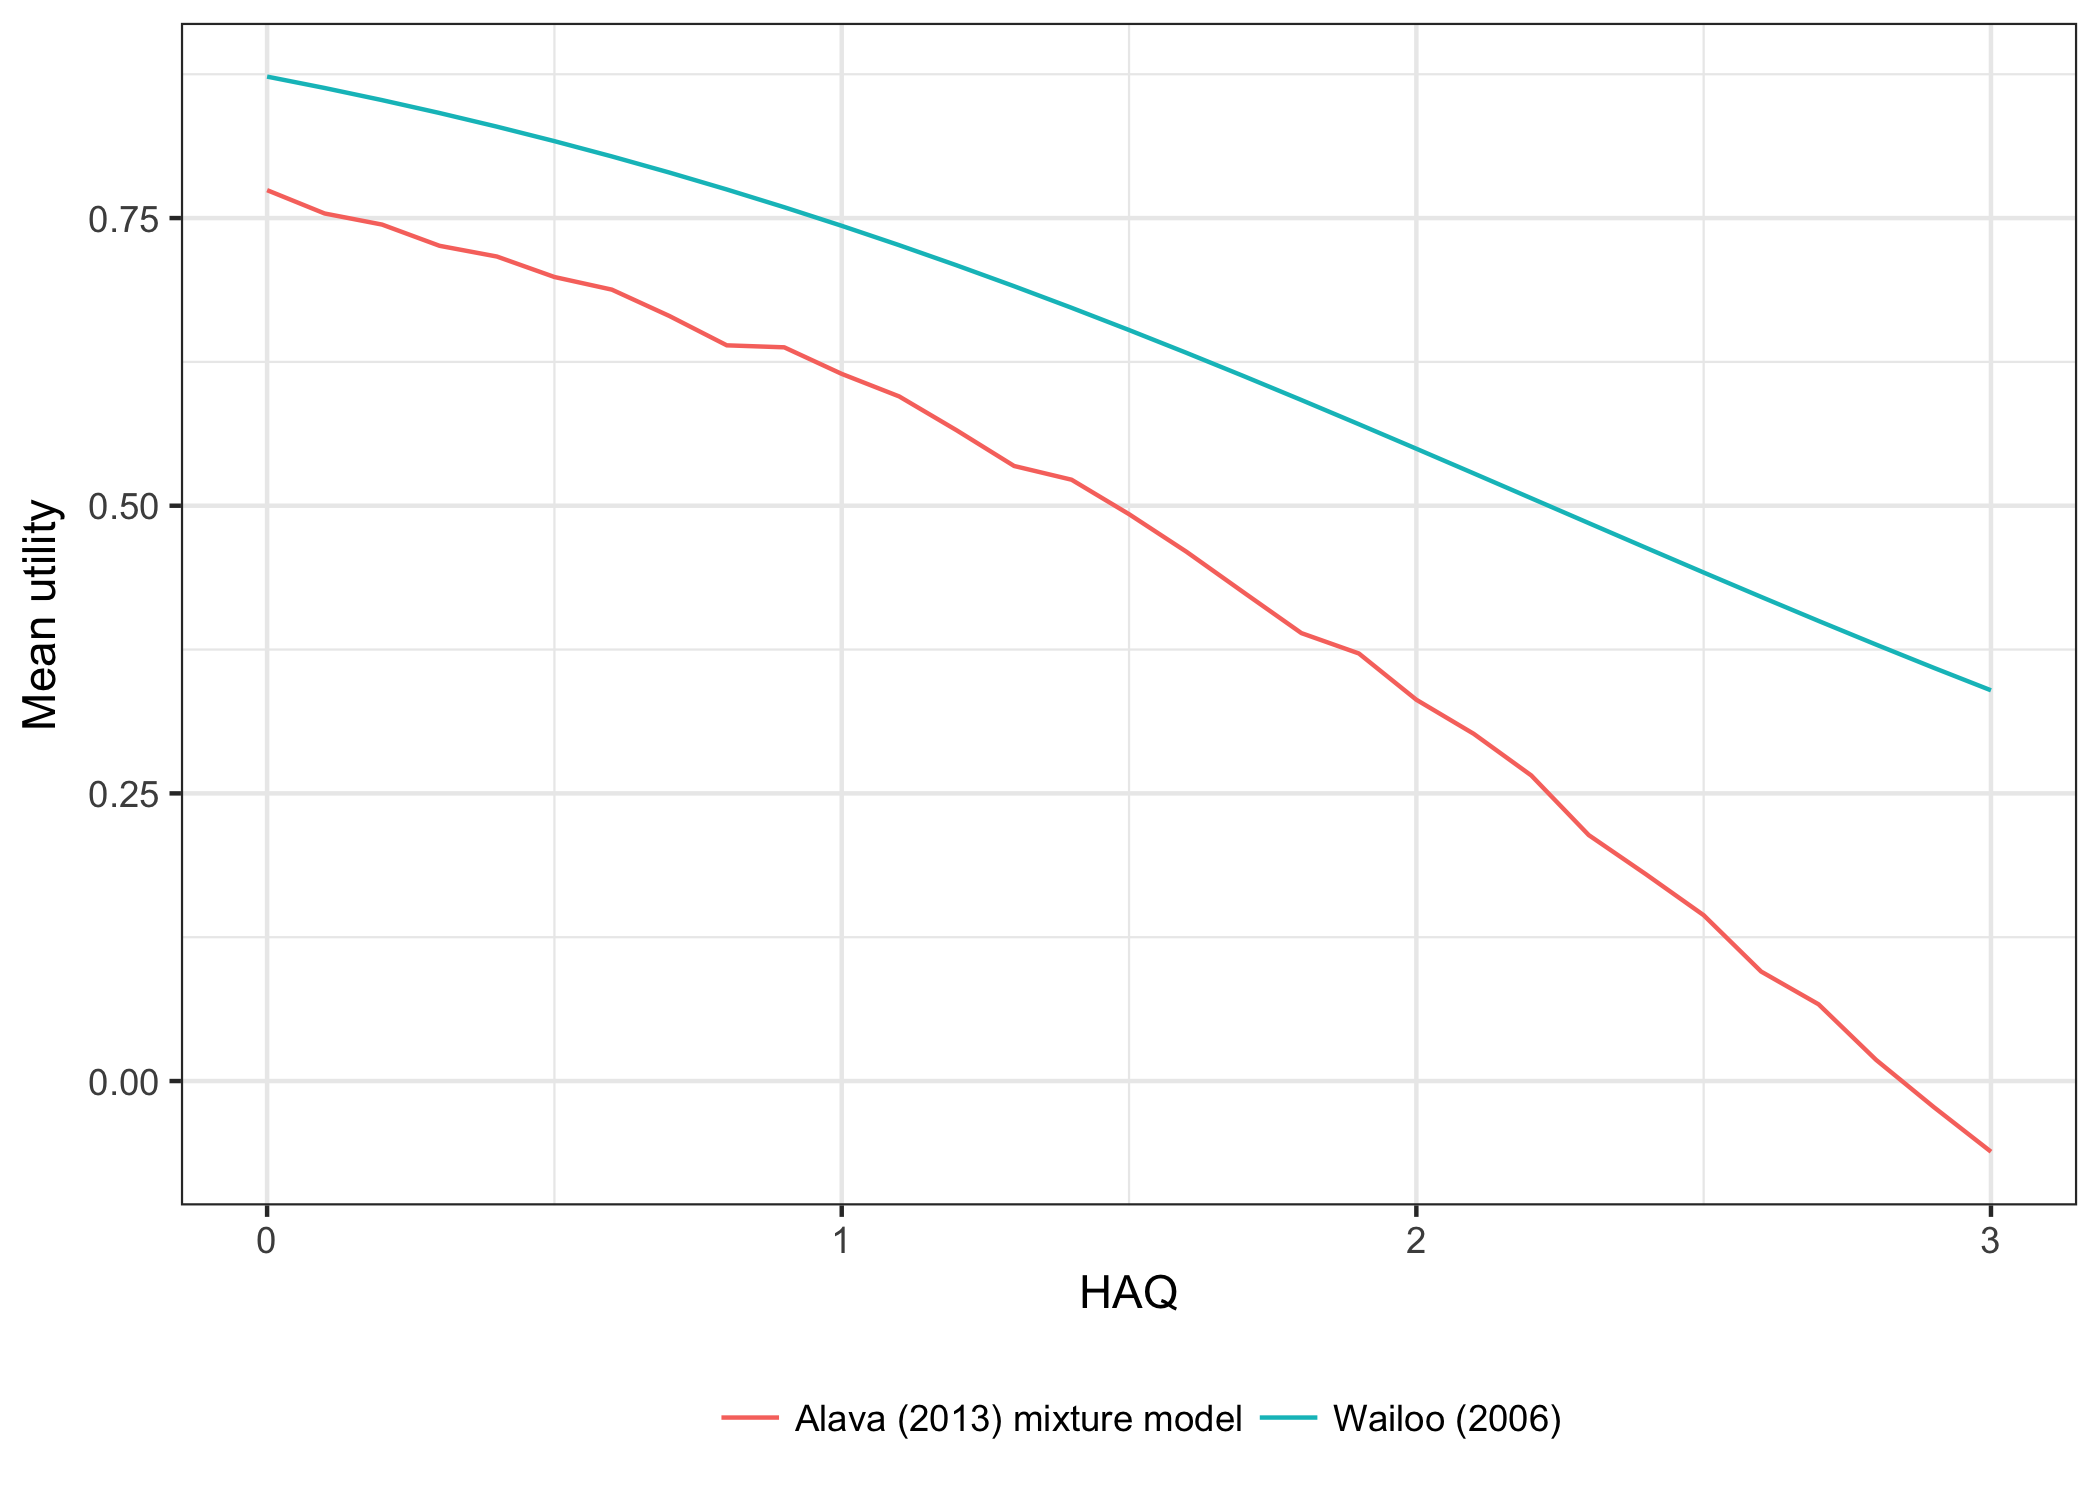
\includegraphics[max size={\textwidth}{\textheight}]{figs/util-byhaq-comparison.png}
\caption{Simulated mean utility by current
HAQ}\label{fig:util-comparison}
\end{figure}

\subsection{Mortality}
The probability of death is simulated as a function of age/sex specific mortality from U.S. lifetables \citep{arias2015united}, baseline HAQ, and changes in HAQ from baseline. \citet{wolfe2003predicting} estimate an odds ratio for the effect of HAQ on mortality of 2.22, which is applied to the absolute mortality rates of the general population (HAQ score of 0). To capture
the effect of treatment on mortality, we assume that, for every 0.25-unit increase in HAQ score, subsequent 6-month mortality increases according to the hazard ratios reported in \citet{michaud2012mortality}.



\begin{table}[!ht]
\begin{center}
\begin{threeparttable}
\caption{Mortality parameters} \label{tbl:mortpars}
\footnotesize
\begin{tabularx}{\textwidth}{@{\extracolsep{\fill}}lcccc}
\hline
\multicolumn{2}{l}{} & \multicolumn{2}{c}{95\% CI} & \multicolumn{1}{l}{} \\
\cmidrule{3-4} 
\multicolumn{1}{l}{} & \multicolumn{1}{l}{Estimate} & \multicolumn{1}{c}{Lower} & \multicolumn{1}{c}{Upper} & \multicolumn{1}{c}{Reference} \\
\hline
Impact of baseline HAQ on mortality \\
\ExpandableInput{tables/mort-or.txt}
Impact of change in HAQ from baseline on mortality\\
\ExpandableInput{tables/mort-hr-haqdif.txt}
\hline
\end{tabularx}
\scriptsize
Notes: 95\% confidence intervals are calculated using normal distributions on the log odds
and log hazard ratio scales. 
\end{threeparttable}
\end{center}
\end{table}

\autoref{fig:surv}



\begin{figure}
\centering
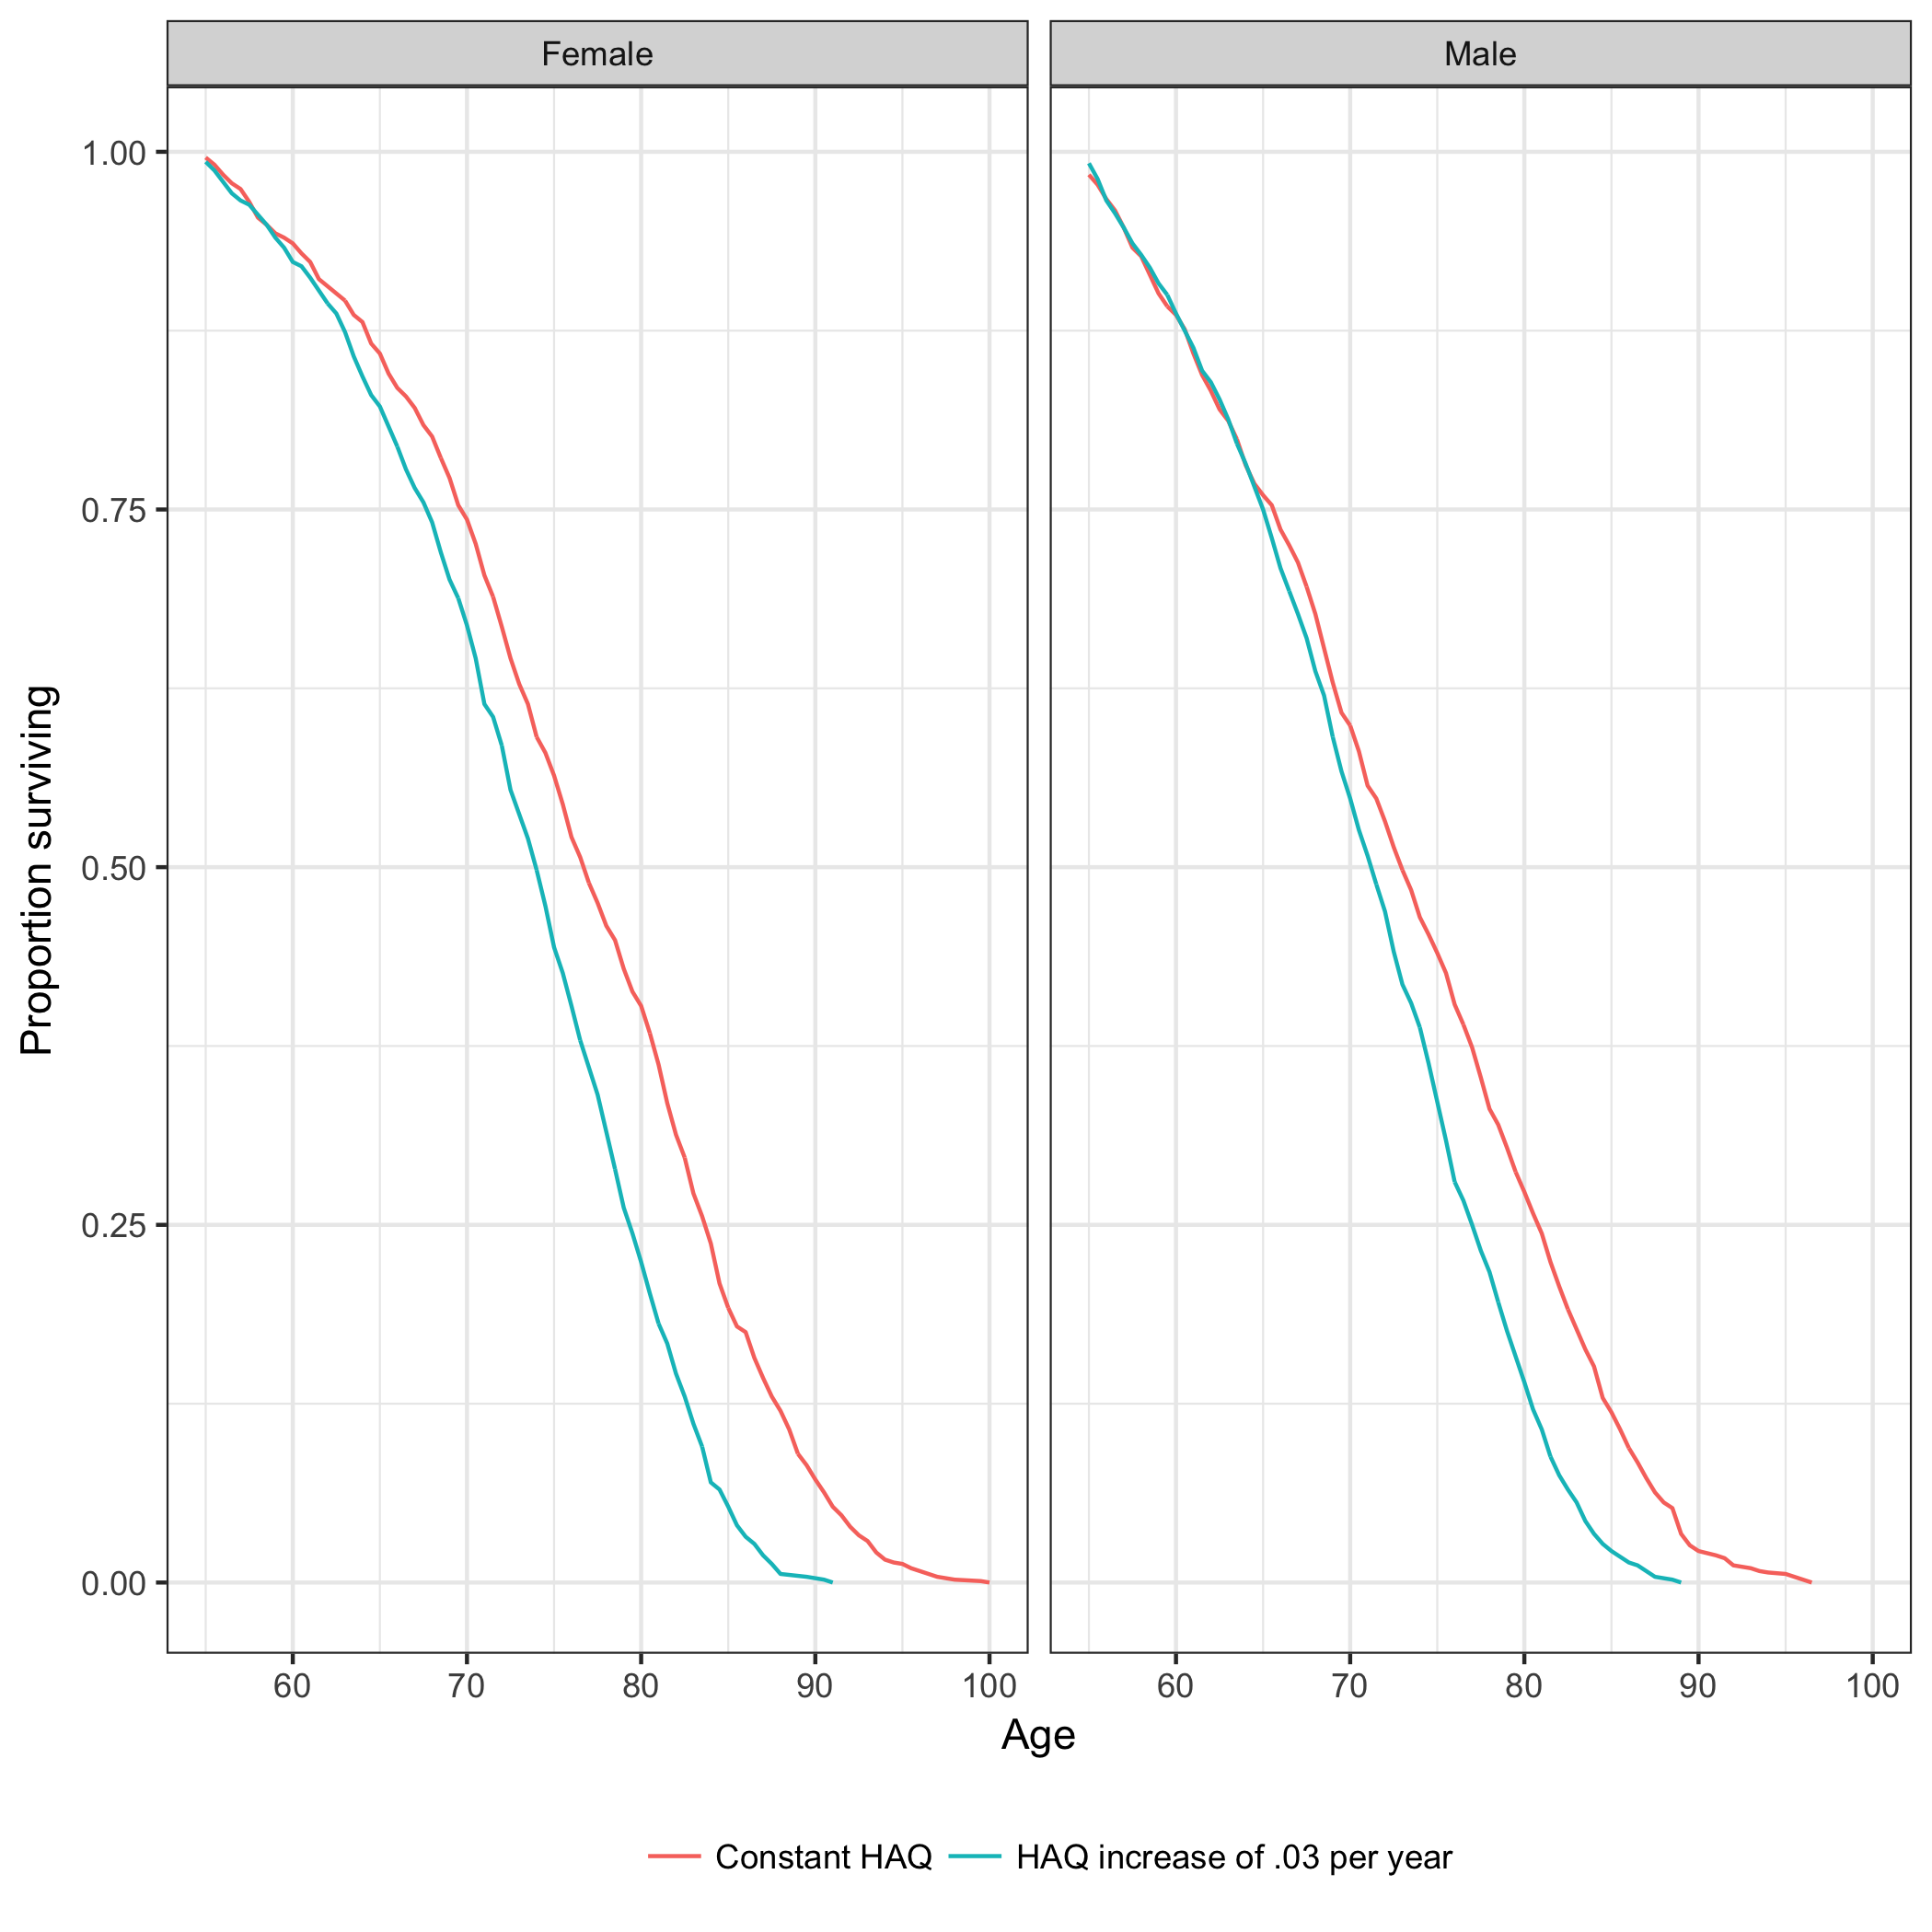
\includegraphics[max size={\textwidth}{\textheight}]{figs/surv.png}
\caption{Simulated survival curve for a patient age 55 with a baseline
HAQ of 1 by change in HAQ per year}\label{fig:surv}
\end{figure}

\subsection{Cost}\label{cost}
Drug costs are based on WACs; discounts can be applied by reducing WACs for specific bDMARDs. Costs related to physician visits, chest X-rays, tuberculosis tests, and inpatient hospital days are based on \citet{claxton2016economic}. The annual number of hospital days relates to the HAQ score according to \citet{carlson2015economic}. Cost of any serious infection are assumed to be equal to the cost of pneumonia hospitalization at \$5,873, based on Medicare reimbursement rates. \citet{wolfe2005household} provide an estimate of annual income loss in relation to HAQ scores: \$4,372 (95\% CI: 2,078 to 6,607; 2002 dollars) change per unit HAQ change. These estimates are inflated to 2016 dollars.



\begin{table}[!ht]
\begin{center}
\begin{threeparttable}
\caption{Resource use parameters} \label{tbl:resource-use-pars}
\footnotesize
\begin{tabularx}{\textwidth}{@{\extracolsep{\fill}}lcccc}
\hline
\multicolumn{2}{l}{} & \multicolumn{2}{c}{95\% CI} & \multicolumn{1}{l}{} \\
\cmidrule{3-4} 
\multicolumn{1}{l}{} & \multicolumn{1}{l}{Estimate} & \multicolumn{1}{c}{Lower} & \multicolumn{1}{c}{Upper} & \multicolumn{1}{c}{Reference} \\
\hline
Days in hospital per year \\
\ExpandableInput{tables/hosp-days-haq.txt}
\ExpandableInput{tables/hosp-cost-perday.txt}
General management cost \\
\ExpandableInput{tables/mgmt-cost.txt}
Productivity loss \\
\ExpandableInput{tables/prod-loss.txt}
\hline
\end{tabularx}
\scriptsize
Notes: 95\% confidence intervals for hospital days per year by HAQ score and hospital cost per day are calculated by using the methods of moments to generate the parameters of the gamma distribution given a mean and standard error. The 95\% confidence intervals for general management costs are based on normal distributions as assumed in \citet{claxton2016economic}. 95\% confidence interval for productivity loss are calculated using a normal distribution and inflated to 2016 dollars. 
\end{threeparttable}
\end{center}
\end{table}



\begin{landscape}
\begin{table}[!ht]
\begin{center}
\begin{threeparttable}
\caption{Drug acquisition and administration cost} \label{tbl:treat-cost}
\scriptsize
\begin{tabular}{lp{0.15\linewidth}p{0.15\linewidth}rrrrrr}
\hline
\multicolumn{1}{l}{Drug} &
\multicolumn{1}{p{0.15\linewidth}}{Dose and frequency of administration} & 
\multicolumn{1}{p{0.15\linewidth}}{Strength and dosage form} & 
\multicolumn{1}{p{0.08\linewidth}}{Number of doses first 6 months}  & 
\multicolumn{1}{p{0.08\linewidth}}{Number of dosees per year beyond the first 6 months} & 
\multicolumn{1}{c}{Wac per unit} & \multicolumn{1}{c}{Infusion cost} & 
\multicolumn{1}{p{0.08\linewidth}}{Cost for the first 6 months} &
\multicolumn{1}{p{0.08\linewidth}}{Cost per year beyond the first 6 months}\\
\hline
\ExpandableInput{tables/treat-cost.txt}
\hline
\end{tabular}
\tiny
Notes: Costs do not include rebates or discounts. Cost for infliximab are calculated by assuming that `r male.prop`\% of patients are male and that the weight of men and women are `r wtmale` kg and `r wtfemale` kg respectively. Tocilizumab is dosed weekly if weight is greater than 100 kg; costs for tocilizumab reported in the table are for patients weighing less than 100 kg. IV = intravenous; SC = subcutaneous; WAC = whoesale acqusition cost. 
\end{threeparttable}
\end{center}
\end{table}
\end{landscape}

\subsection{Patient preferences for treatment
attributes}\label{patient-preferences-for-treatment-attributes}

\section{Simulation and uncertainty analysis}\label{sec:sim-uncertainty}

\subsection{Individual patient simulation}\label{individual-patient-simulation}

The IPS is a discrete-time simulation that simulates individual patients one at a time. Model cycle, denoted by $t$, were chosen to be 6-months long to be consistent with most RCT and real-world data evidence. \autoref{alg:IPS} describes the main components of the IPS for a single patient and a given treatment in a treatment sequence. The full simulation cycles through each treatment in a sequence and through each simulated patient.

\begin{algorithm}
\caption{Main components of the individual patient simulation}
\label{alg:IPS}
\begin{enumerate}
\item \textbf{Initial treatment effect ($t = 0$)}
\begin{enumerate}
\item Simulate clinical response (SDAI or EULAR), time to serious infection $T_{si}$, and death.
\begin{enumerate}
\item \textbf{If} no clinical response, \textbf{then} stop treatment. Treatment switch caused by a serious infection if time to serious infection occured during cycle 0 (i.e. $T_{si} = 0$). Change in HAQ is assumed to be $0$. 
\newline \textbf{Else if} clinical response, \textbf{then} continue treatment. Simulate change in HAQ and time to treatment discontinuation $T$.
\item \textbf{If} patient died, \textbf{then} move to next patient. 
\end{enumerate}
\end{enumerate}
\item \textbf{Maintenance phase} (for $t > 0 \text{ and } t \leq T$)
\begin{enumerate}
\item Simulate death (see \autoref{ssec:simulating-death}) and change in HAQ.
\item \textbf{If} patient died, \textbf{then} move to next patient.
\item \textbf{If} $t = T$, \textbf{then} switch treatment. Treatment switch caused by a serious infection if time to serious infection occured during or before cycle T (i.e. $T_{si} \leq T$). 
\end{enumerate}
\end{enumerate}
\end{algorithm}

\subsection{Parameter uncertainty}\label{parameter-uncertainty}
Parameter uncertainty is quantified using PSA, which propagates uncertainty in the model input parameters throughout the model by randomly sampling the input parameters from their joint probability distribution. Probability distributions are determined according to the distributional properties of the statistical estimates, which, in turn, depend on the statistical techniques used and the distributions of the underlying data. The probability distribution used for each parameter in our model is shown in Table ?. In addition, the table summarizes the mean, standard deviation, and 2.5\% and 97.5\% quantiles from a random sample of size 1,000 from the joint probability distribution.   

\subsection{Structural uncertainty}\label{stuctural-uncertainty}

\subsection{Implementation}\label{implementation}

\begin{appendices}

\section{Individual Patient Simulation}\label{appendix:IPS}
\subsection{Non-linear HAQ trajectory}\label{non-linear-haq}
\citet{norton2014health} model HAQ progression using a latent class growth model (LCGM). The probability that individual $i$ is a member of class $c$ at time $t$ is modeled using a multinomial logistic regression
\begin{align}
P(C_{it} = c) &= \frac{\exp(w_{it}^T\delta_c)}{\sum_{s=1}^{4}\exp(w_{it}^T\delta_s)},
\end{align}
where $\delta_s$ is the vector of regression coefficeints associated with class $s$ and $w_i$ is the corresponding design matrix for individual $i$. The variables included in $w_i$ are age, gender, baseline DAS28, symptom duration, rheumatoid factor, ACR criteria, and socieoeconomic status. 

\subsection{Effect of age on linear HAQ
progression}\label{effect-of-age-on-linear-haq-progression}

\subsection{Simulating death}\label{ssec:simulating-death}
Death is simulated for each patient during each model cycle based on age, gender, baseline HAQ, and change in HAQ from baseline. A 0/1 death indicator is randomly drawn using the following procedure: 
\begin{enumerate}
\item Use the annual probability of death ($q_x$) from lifetables based on patient age and gender.
\item Adjust the probability of mortality, $p_m$, using odds of mortality, $OR$, of a change in baseline HAQ.
\begin{align}
p_m = \frac{1}{1 + \exp{\left[-(\log(q_x) + HAQ \cdot \log(OR))\right]}}
\end{align}
\item Convert the mortality probability, $p_m$, into a mortality rate, $r_m$.
\begin{align}
r_m &= -log(1 - p_m)
\end{align}
\item Adjust the mortality rate using the estimated hazard ratio of mortality, $HR$ of a change in HAQ from baseline, $\Delta$ HAQ.
\begin{align}
r_m &= r_m \cdot \exp[\log(HR) \cdot \Delta HAQ]
\end{align}
\item Convert the mortality rate into a probability given a 6-month cycle length.
\begin{align}
p_m = 1 - \exp[-r_m * (6/12)]
\end{align}
\item Randomly draw a 0/1 death indicator, $d$, given the probability of death, $p_m$.
\begin{align}
d \sim \text{Bin}(1, p_m)
\end{align}
\end{enumerate}

\subsection{Simulating utility}\label{simulating-utility}
\subsubsection{Mixture model}
Utiliy was simulated in a two stages using the mixture model estimated by \citet{alava2013relationship}. In the first stage, we sampled pain for a given individual in a particular model cycle based on the HAQ score. In the second stage, we simulated utility as a function of HAQ, pain and age/sex.

\textbf{Simulating pain}\\
To simulate pain from HAQ, we used the summary statistics for pain and HAQ reported in \citet{sarzi2002correlation}. Pain was measured with the visual analog scale (VAS) with mean  $\mu_{pain} =$ 61.65 and standard deviation $\sigma_{pain} =$ 19.10, while HAQ was reported to have mean $\mu_{haq} =$ 1.39 and standard deviation $\sigma_{haq} =$ 0.59. 

We then estimated the correlation between pain and HAQ by digitally scanning the curve depicting the (linear) relationship between pain and HAQ (Figure 114) shown in \citet{stevenson2016adalimumab}. Using the scanned data, we regressed pain on HAQ using simple ordinary least squares (OLS). The correlation between pain and HAQ, estimated as $\rho =$ 0.52, was calculated by rearranging the OLS estimate for the slope, $\beta$, of the regression model,

\begin{align}
\rho = \beta \cdot \frac{\sigma_{haq}}{\sigma_{pain}}.
\end{align}

Pain was simulated using these parameters by assuming that pain was normally distributed conditional on HAQ,

\begin{align}
pain | haq = h \sim N\left (\mu_{pain} + \rho \frac{\sigma_{pain}}{\sigma_{haq}}(h - \mu_{haq}), \sigma^2_{pain}(1 - \rho^2)\right).
\end{align}

However, since the VAS is constrained to lie between 0 and 100, pain was drawn from a truncated normal distribution with a lower limit of 0 and an upper limit of 100. 


\textbf{Simulating utility}\\
After simulating pain, we simulated utility with a mixture model. Within each class $c$, the HAQ score for patient $i$ in period $t$ was modeled as,

\begin{align}
y_{it|C_{it}} &= 
\begin{cases}
  1 & \text{if}\  y^{*}_{it|C_{it}}>0.883 \\
  y^{*}_{it|C_{it}} & \text{otherwise}
\end{cases}\\
y^{*}_{it|C_{it}} &= \alpha_{ic} +  x_{it}^T\beta_{c} + \epsilon_{it}\\
\alpha_{ic} &= \gamma_{ic} + z_{i}^T\gamma_{i}^{0} + \mu_{i}
\end{align}

The probability of class membership was modeled using a multinomial logit model,

\begin{align}
P(C_{it} = c) &= \frac{\exp(w_{it}^T\delta_c)}{\sum_{s=1}^{4}\exp(w_{it}^T\delta_s)}.
\end{align}

We sampled from the mixture model as follows.

\begin{enumerate}
\item For each individual $i$, sample the error term, $\mu_{i} \sim N(0, \sigma^2_\mu)$.
\end{enumerate}


\subsubsection{Wailoo utility algorithm}\label{Wailoo-utility}

\section{Network Meta-Analysis}\label{appendix:NMA}

\subsection{Bayesian NMA for initial treatment
effects}\label{sec:tech-nma-initial}

\subsubsection{Systematic literature
review}\label{systematic-literature-review}

\textbf{Population}
\begin{itemize}
\item
  Adult (\textgreater{}18 years) patients with moderate to severe RA who
  have had inadequate response to cDMARDs
\end{itemize}

\textbf{Interventions and comparators}

\begin{itemize}
\item
  Biologics as monotherapy or in combination with cDMARDs (adalimumab,
  certolizumab pegol, etanercept, golimumab, infliximab, abatacept,
  rituximab, tocilizumab, sarilumab, tofacitinib, baricitinib)
\item
  Triple therapy (MTX, HCQ, and SSZ)
\item
  cDMARDs alone or in combination (MTX, HCQ, SSZ or LEF)
\end{itemize}

\textbf{Outcomes}
\begin{itemize}
\item
  ACR20/ACR50/ACR70
\item
  DAS28
\item
  Total sharp score
\item
  HAQ-DI score
\item
  SF-36 PCS and MCS
\item
  EQ-5D (VAS and utility scores)
\item
  AEs leading to drop-outs
\end{itemize}

\begin{itemize}
\item
  Randomized controlled trials
\end{itemize}

\textbf{Other}

\begin{itemize}
\item
  Studies published in English
\item
  Primary study available as full text published manuscript only; no
  study available as a conference abstract only was included with the
  exception of abstracts pertaining to investigational products,
  baricitinib and sarilumab
\end{itemize}

\subsubsection{Criteria for studies to be selected from the systematic
literature review and included in the
NMA}\label{criteria-for-studies-to-be-selected-from-the-systematic-literature-review-and-included-in-the-nma}

The following criteria were used to select relevant studies to be
included in the NMA:

\textbf{Population}

\begin{itemize}
\item
  Adult (\textgreater{}18 years) patients with moderate to severe RA who
  have had inadequate response to cDMARDs and are bDMARD-naive
\end{itemize}

\textbf{Interventions}

\begin{itemize}
\item
  Biologics as monotherapy or in combination with cDMARDs (adalimumab,
  certolizumab pegol, etanercept, golimumab, infliximab, abatacept,
  rituximab, tocilizumab, sarilumab, tofacitinib, baricitinib)
\end{itemize}

\textbf{Comparators}

\begin{itemize}
\item
  cDMARDs
\item
  Any active comparator that allows for an indirect comparison between
  the bDMARDs of interest
\end{itemize}

\textbf{Outcomes}

\begin{itemize}
\item
  ACR20/ACR50/ACR70 at 6 months follow-up
\end{itemize}

\subsubsection{Identified evidence base}\label{identified-evidence-base}

\autoref{fig:study-selection} summarizes the study identification and
selection process. Of the 181 studies included in the large systematic
literature review, 79 studies concerned the bDMARD-naive population
(table NMA studies). There were 66 studies evaluating 36 interventions
for which ACR response criteria were reported at 6 months (with a
tolerability window of \(\pm 4\) weeks). The corresponding evidence
network is presented in \autoref{fig:nma-network-acr-naive}. For the
network meta-analysis the following were deemed to be clinically
equivalent and were pooled.

\begin{itemize}
\item
  ``INF 3mg/kg q8w'' or ``INF 5mg/kg q8w'' or ``INF 6mg/kg q8w''
\item
  ``ETN 50mg qw'' or ``ETN 25mg biw''
\item
  ``ABA 10mg/kg q4wa or''ABA SC 125mg qw"
\item
  ``CER 200mg q2w+MTX'' or ``CER 400mg q4w+MTX
\item
  DMARDs including methotrexate, sulfasalazine, hydroxychloroquine,
  leflunomide at any dosage; studies which only described DMARD therapy
  as conventional or nonbiologic
\end{itemize}

\begin{figure}
\centering
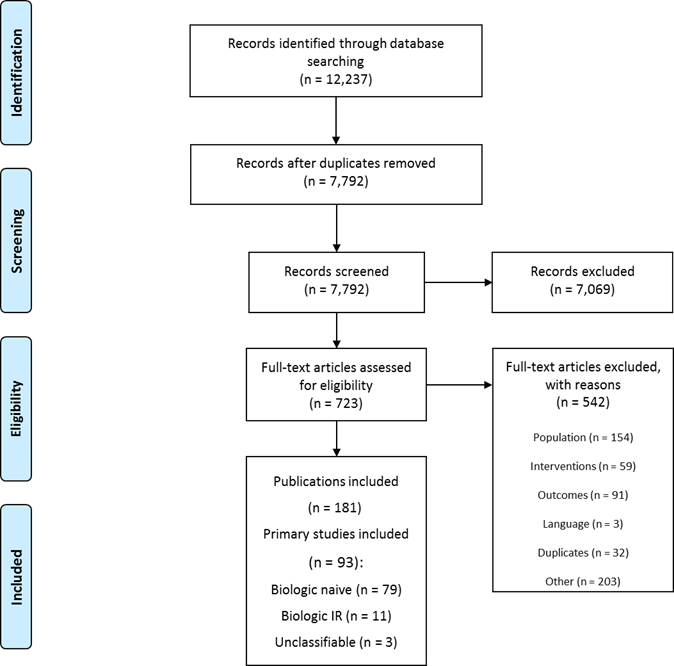
\includegraphics[max size={\textwidth}{\textheight}]{figs/study-selection.png}
\caption{Study identification and selection}\label{fig:study-selection}
\end{figure}

\begin{figure}
\centering
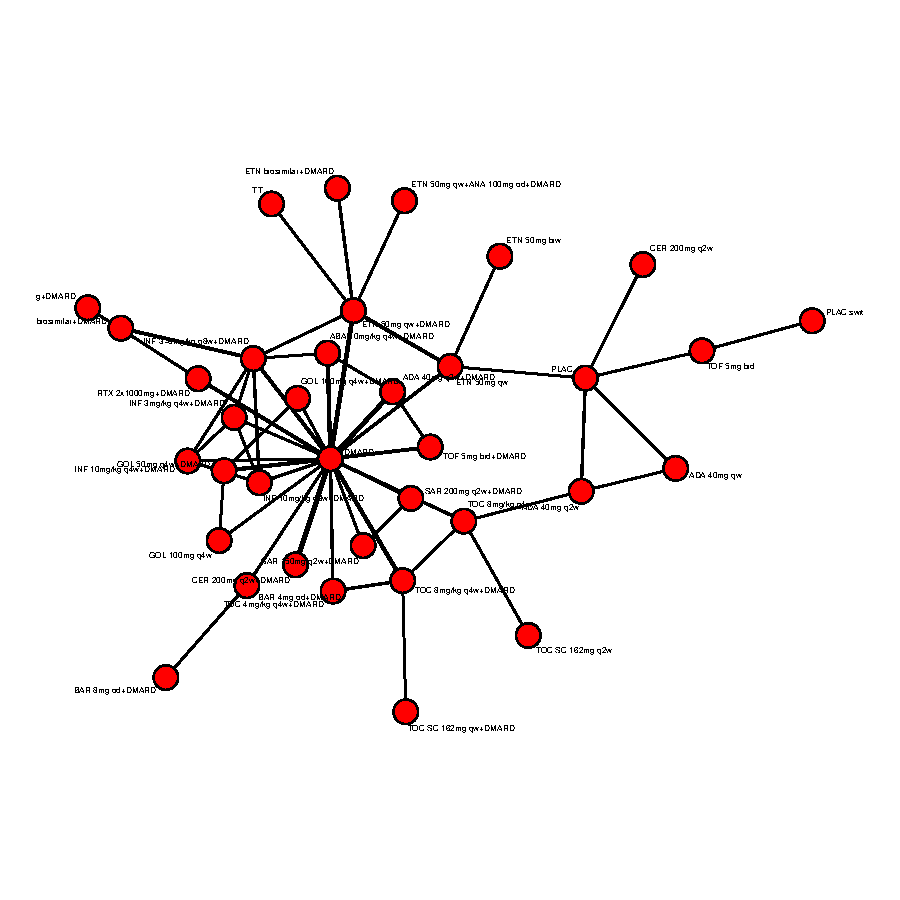
\includegraphics{figs/nma-network-acr-naive.pdf}
\caption{Bayesian random effects NMA network diagram for patients naive
to bDMARDs}\label{fig:nma-network-acr-naive}
\end{figure}

\subsubsection{Network meta-analysis to obtain ACR 20/50/70
response}\label{network-meta-analysis-to-obtain-acr-205070-response}

The probability of ACR20/50/70 responses was estimated using a Bayesian (random effects) network meta-analyses model for ordered categorical data \citep{dias2013evidence}. The model assumes that there is an underlying continuous variable (ACR20/50/70) categorized by specifying different cutoffs corresponding to the point at which an individual moves from one category to the next in each trial. The advantage of this approach over an analysis that considers ACR categories separately is that all possible outcomes are analyzed simultaneously based on the same randomized controlled trials, allowing for consistent estimates by category. To avoid influencing the observed results by prior belief, uninformative prior distributions were used for the estimated model parameters. The relative treatment effects for each bDMARD versus cDMARDs estimated on the probit scale were transformed into absolute probabilities of the nonoverlapping ACR response categories by combining them with the average results for cDMARDs. The posterior distributions of parameters of interest were summarized by the median as a reflection of the point estimate and 95\% credible intervals, constructed from the 2.5 and 97.5 percentiles. Analyses were performed with the Markov chain Monte Carlo method using the JAGS software package (\url{http://mcmc-jags.sourceforge.net/}).

\subsection{Network meta-analysis to obtain
HAQ}\label{network-meta-analysis-to-obtain-haq}

\end{appendices}

\pdfbookmark[1]{References}{References}
\bibliography{../../vignettes/vignettes}

\end{document}
